\section{Introduction}


Parking lots present a difficult search problem. Drivers lack the visibility
to determine where spots are available, and may spend a non-trivial amount of
time searching for a spot. The problem is difficult enough that WikiHow
includes directions~\cite{wikihow-park}, and the Wall Street Journal has
published an online article~\cite{wsj-park} with tips on spot stalking for
shoppers during the holidays. Searching not only generates frustration but
also wastes energy and produces harmful carbon emissions.

Online smartphone application stores such as Google Play and the App Store
are teeming with apps claiming to help you find a parking spot. Although some
drivers may find these applications useful, they either do not provide
real-time parking lot availability or simply display publicly-available
information. Several research projects have attempted to address these
limitations~\cite{4212497, Chen:2012:COS, Delot:2009:CRP, 5062057,
Mathur:2010:PDS}, but include requirements rendering them impractical, such
as additional infrastructure~\cite{5062057}, on-vehicle
equipment~\cite{Mathur:2010:PDS} or vehicular
networking~\cite{Delot:2009:CRP, Mathur:2010:PDS}, or onerous manual user
input~\cite{Chen:2012:COS}. In contrast, we believe the solution is already
in your pocket.

We present \textit{PocketParker}, a system that predicts parking lot
availability using smartphones. Unlike previous approaches, PocketParker
requires no additional infrastructure, no vehicle modifications, and no user
input, only installation on a small percentage of the 100~million smartphones
already in use in the US~\cite{smartphone-numbers}. PocketParker runs
unattended in the background and uses the accelerometer to detect parking lot
arrivals and departures.  These are forwarded to a central server, which
incorporates them into per-lot availability models.  This allows PocketParker
to order lots accurately by the probability that they contain an available
spot.  In general, we consider our approach to be an example of a subset of
crowdsourcing that does not require any manual user input, which we call
\textit{pocketsourcing}.

Providing parking availability predictions requires efficiently and
accurately detecting parking-related events, and incorporating the effect of
\textit{hidden drivers}---those not using PocketParker---into our
availability model. We address the first challenge by designing a simple yet
effective event detector which uses the smartphone accelerometer to
efficiently detect arrival and departure events, triggering energy-hungry GPS
acquisition only when necessary. We address the second challenge by designing
an availability estimator that maintains a probability model for each lot
continuously incorporating data from PocketParker clients. We use detected
events both to estimate arrival and departure rates and to make changes in
real time. Part of the key to our approach is the observation that even with
limited information, there are moments when PocketParker can be certain about
the availability of a parking spot in a given lot, and this certainty allows 
PocketParker to assist users.

We perform a careful evaluation of PocketParker using a variety of methods
tailored to each system component. We evaluate our parking event detector in
a controlled environment with eight volunteers participating in ten parking
scenarios. We design a simulator to evaluate our parking availability
estimator, which gives us the flexibility to experiment with a variety of
parameters and parking lot types. Finally, we evaluate the overall
effectiveness of PocketParker by deploying it with 105 smartphones used by
our participants over forty five days. To obtain ground truth, we deploy four
cameras that monitor two parking lots over two weeks. We inspect and
hand-code four days' worth of images of these lots to measure their true
availability. Altogether, our results show the efficiency and accuracy
of PocketParker.

As depicted in Figure~\ref{fig-arch}, PocketParker has several components
distributed across participating smartphones and a backend server. The rest
of our paper describes each component in detail. We start by presenting
related work in Section~\ref{sec-related} in order to distinguish
PocketParker from multiple previous efforts at parking monitoring. Next, in
Sections~\ref{sec-detector}~and~\ref{sec-model} we describe two major 
components of PocketParker: our parking event detector and availability
model.  We base our evaluation in Section~\ref{sec-evaluation} on simulations
and controlled exeriments stemming from two real-world deployments.  Finally,
we discuss limitations and future work in Section~\ref{sec-future} before
concluding in Section~\ref{sec-conclusions}.

\begin{figure}
\centering
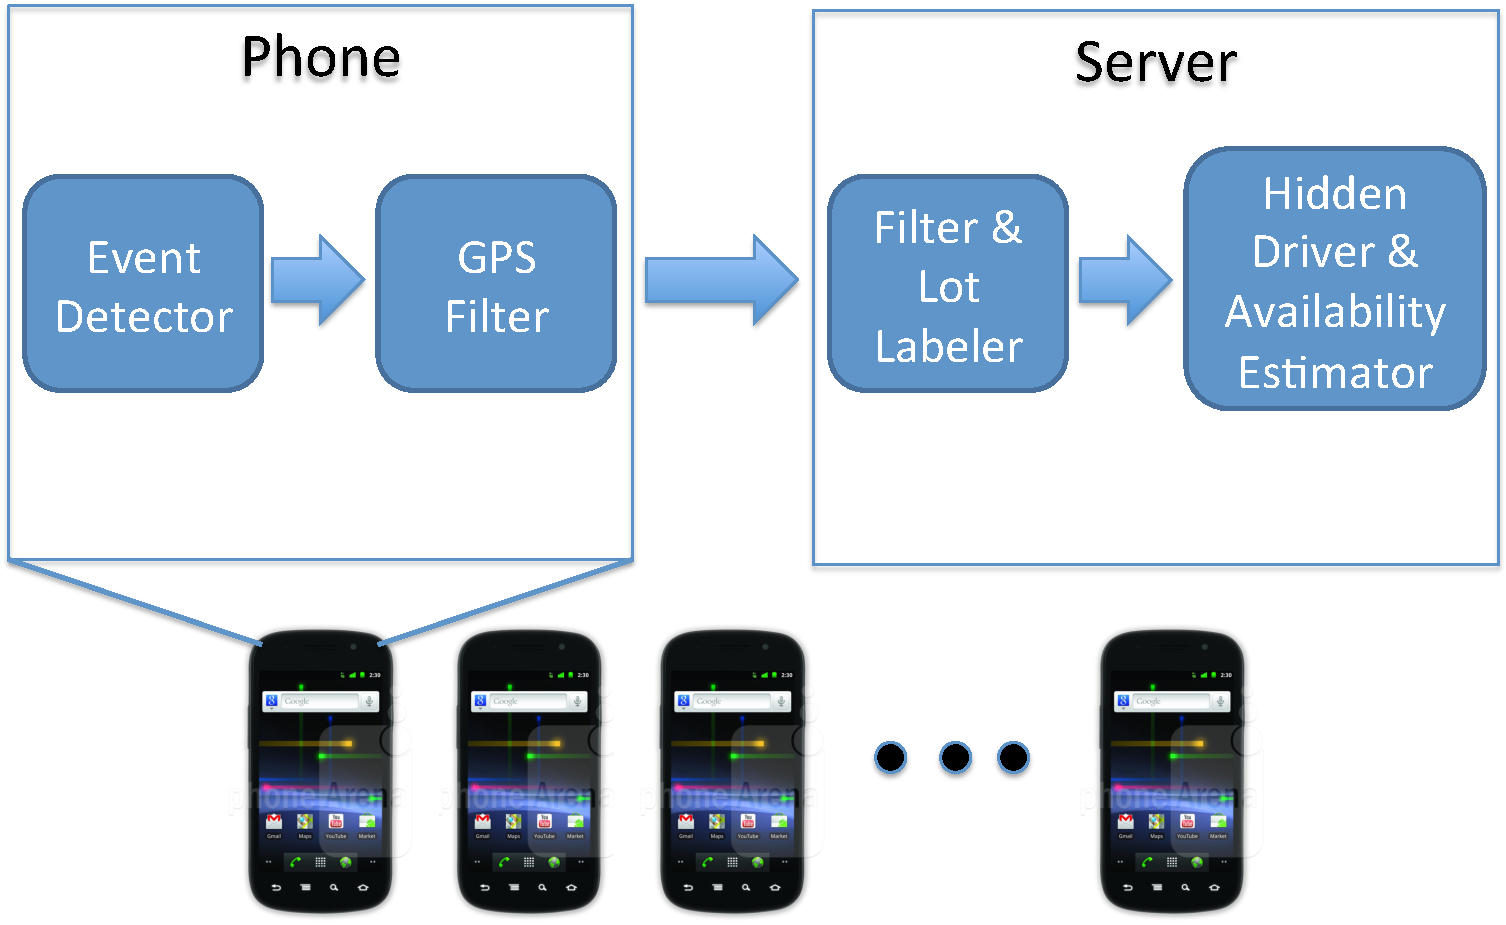
\includegraphics[height=1.5in]{./figures/blockdiagram.pdf}

\caption{\textbf{The PocketParker architecture.} Events generated by an
activity detector running quietly on each smartphone are processed by a
central server and used to estimate parking lot availability.}

\label{fig-arch}
\vspace*{-0.2in}
\end{figure}
